\section{Preventivo} 
	\subsection{Introduzione}
		A fronte della pianificazione sono stati decise per ogni fase quante ore ogni componente del gruppo dovrà svolgere per ruolo.
		Per favorire la rotazione dei ruoli sarà possibile che alcuni membri in una singola fase svolgano diversi ruoli. \\
		Nelle tabelle e in alcuni grafici si farà uso delle abbreviazioni seguenti per indicare i ruoli:
		\begin{itemize}
			\item RE: Responsabile;
			\item AM: Amministratore;
			\item AN: Analista;
			\item PG: Progettista;
			\item PR: Programmatore;
			\item VR: Verificatore.
		\end{itemize}
		
	\subsection{Fase non rendicontanta}
		
		\subsubsection{Fase A}
		
			\paragraph{Suddivisione del lavoro}
			Nella seguente tabella è descritta la divisione del lavoro nella fase A:
			\begin{tabella}{!{\VRule}c!{\VRule}c!{\VRule}c!{\VRule}c!{\VRule}c!{\VRule}c!{\VRule}c!{\VRule}c!{\VRule}}
				
				\intestazioneeightcol{Nome}{RE}{AM}{AN}{PG}{PR}{VR}{Ore totali}
				
				Viviana Alessio & 12 & 2 & - & - & - & 8 & 22 \\
				Enrico Bellio & - & - & 15 & - & - & 7 & 22 \\
				Matteo Franco & - & 14 & - & - & - & 8 & 22 \\
				Andrea Grendene & - & - & 20 & - & - & 3 & 23 \\
				Tommaso Panozzo & - & 6 & 15 & - & - & 3 & 24 \\
				Luca Soldera  & - & 14 & - & - & - & 8 & 22 \\
				
				\hiderowcolors
				\caption{Ore per componente - Fase A}
				
			\end{tabella}
			\newpage
			
			Vengono esposti visivamente i dati riportati in tabella attraverso il seguente istogramma:
			\ist{img/istogrammiOre/istA}{Istogramma ruoli - Fase A}
			
			
			\paragraph{Prospetto economico}
			I costi di questa fase non vengono rendicontati al Proponente. Nella seguente tabella sono riportati i costi relativi alla fase A: 
			\begin{tabella}{!{\VRule}c!{\VRule}c!{\VRule}c!{\VRule}}
				\intestazionethreecol{Ruolo}{Ore}{Costo}
				
				Responsabile & 12 & 360\euro \\
				Amministratore & 36 & 720\euro \\
				Analista & 50 & 1250\euro \\
				Progettista & - & - \\
				Programmatore & - & - \\
				Verificatore & 37 & 555\euro \\
				\hline
				\textbf{Totale} & \textbf{135} & \textbf{2885\euro} \\
				\hiderowcolors
				\caption{Ore per ruolo - Fase A}
			\end{tabella}	
			\newpage
			
			\torta{img/percSoldi/percSoldiA.png}{Percentuale di costo per ruolo sul totale - Fase A}	
			\torta{img/percOre/PercentualeOreFaseA.png}{Percentuale di ore per ruolo sul totale - Fase A}

	\newpage		
	\subsection{Fasi rendicontate}
	
		\subsubsection{Fase AD}
			\paragraph{Suddivisione del lavoro}
			Nella seguente tabella è descritta la divisione del lavoro nella fase AD: \\ \\
			\begin{tabella}{!{\VRule}c!{\VRule}c!{\VRule}c!{\VRule}c!{\VRule}c!{\VRule}c!{\VRule}c!{\VRule}c!{\VRule}}
				
				\intestazioneeightcol{Nome}{RE}{AM}{AN}{PG}{PR}{VR}{Ore totali}
				
				Viviana Alessio & - & - & 10 & - & - & - & 10 \\
				Enrico Bellio & - & - & - & - & - & 10 & 10 \\
				Matteo Franco & - & - & 10 & - & - & - & 10 \\
				Andrea Grendene & - & 3 & - & - & - & 7 & 10 \\
				Tommaso Panozzo & - & 5 & 5 & - & - & - & 10 \\
				Luca Soldera  & 5 & - & 5 & - & - & - & 10 \\
				
				\hiderowcolors
				\caption{Ore per componente - Fase AD}
				
			\end{tabella}
			
			
			\ist{img/istogrammiOre/istAD}{Istogramma ruoli - Fase AD}

			
			\paragraph{Prospetto economico}
			Nella seguente tabella sono riportati i costi relativi alla fase AD da rendicontare al Proponente: 
			\begin{tabella}{!{\VRule}c!{\VRule}c!{\VRule}c!{\VRule}}
				\intestazionethreecol{Ruolo}{Ore}{Costo}
				
				Responsabile & 5 & 150\euro \\
				Amministratore & 8 & 160\euro \\
				Analista & 30 & 750\euro \\
				Progettista & - & - \\
				Programmatore & - & - \\
				Verificatore & 17 & 255\euro \\
				\hline
				\textbf{Totale} & \textbf{60} & \textbf{1315\euro} \\
				\hiderowcolors
				\caption{Ore per ruolo - Fase AD}
				\end{tabella}	
			
			\torta{img/percSoldi/percSoldiAD.png}{Percentuale di costo per ruolo sul totale - Fase AD}	
			\torta{img/percOre/PercentualeOreFaseAD.png}{Percentuale di ore per ruolo sul totale - Fase AD}
		\newpage
		\subsubsection{Fase PA}
			\paragraph{Suddivisione del lavoro}
			Nella seguente tabella è descritta la divisione del lavoro nella fase PA:
			\begin{tabella}{!{\VRule}c!{\VRule}c!{\VRule}c!{\VRule}c!{\VRule}c!{\VRule}c!{\VRule}c!{\VRule}c!{\VRule}}
				
				\intestazioneeightcol{Nome}{RE}{AM}{AN}{PG}{PR}{VR}{Ore totali}
				
				Viviana Alessio & - & 5 & 10 & - & - & 20 & 35 \\
				Enrico Bellio & - & 5 & 10 & - & - & 20 & 35 \\
				Matteo Franco & - & - & - & 23 & - & 10 & 33 \\
				Andrea Grendene & - & - & - & 20 & - & 15 & 35 \\
				Tommaso Panozzo & 10 & - & - & 23 & - & - & 33 \\
				Luca Soldera  & - & - & - & 25 & - & 10 & 35 \\
				
				\hiderowcolors
				\caption{Ore per componente - Fase PA}
				
			\end{tabella}

			\newpage
			
			\ist{img/istogrammiOre/istPA}{Istogramma ruoli - Fase PA}
			
			\paragraph{Prospetto economico}
			Nella seguente tabella sono riportati i costi relativi alla fase PA da rendicontare al Proponente: 
			\begin{tabella}{!{\VRule}c!{\VRule}c!{\VRule}c!{\VRule}}
				\intestazionethreecol{Ruolo}{Ore}{Costo}
				
				Responsabile & 10 & 300\euro \\
				Amministratore & 10 & 200\euro \\
				Analista & 20 & 500\euro \\
				Progettista & 91 & 2002\euro \\
				Programmatore & - & - \\
				Verificatore & 75 & 1125\euro \\
				\hline
				\textbf{Totale} & \textbf{206} & \textbf{4127\euro} \\
				\hiderowcolors
				\caption{Ore per ruolo - Fase PA}
				\end{tabella}
			\newpage
			
			\torta{img/percSoldi/percSoldiPA.png}{Percentuale di costo per ruolo sul totale - Fase PA}	
			\torta{img/percOre/PercentualeOreFasePA.png}{Percentuale di ore per ruolo sul totale - Fase PA}
			\newpage
		
		\subsubsection{Fase PDC}
			\paragraph{Suddivisione del lavoro}
			Nella seguente tabella è descritta la divisione del lavoro nella fase PDC:
			\begin{tabella}{!{\VRule}c!{\VRule}c!{\VRule}c!{\VRule}c!{\VRule}c!{\VRule}c!{\VRule}c!{\VRule}c!{\VRule}}
				
				\intestazioneeightcol{Nome}{RE}{AM}{AN}{PG}{PR}{VR}{Ore totali}
				
				Viviana Alessio & - & - & - & 14 & 15 & 8 & 37 \\
				Enrico Bellio & - & - & - & - & 23 & 10 & 33 \\
				Matteo Franco & 10 & - & 6 & 8 & - & 11 & 35 \\
				Andrea Grendene & - & - & - & - & 25 & 10 & 35 \\
				Tommaso Panozzo & - & - & - & 13 & 15 & 7 & 35 \\
				Luca Soldera  & - & 5 & 3 & 10 & 3 & 13 & 34 \\
				
				\hiderowcolors
				\caption{Ore per componente - Fase PDC}
				
			\end{tabella}
			
			\ist{img/istogrammiOre/istPDC}{Istogramma ruoli - Fase PDC}
			
			
			\paragraph{Prospetto economico}
			Nella seguente tabella sono riportati i costi relativi alla fase PDC da rendicontare al Proponente: 
			\begin{tabella}{!{\VRule}c!{\VRule}c!{\VRule}c!{\VRule}}
				\intestazionethreecol{Ruolo}{Ore}{Costo}
				
				Responsabile & 10 & 300\euro \\
				Amministratore & 5 & 100\euro \\
				Analista & 9 & 225\euro \\
				Progettista & 45 & 990\euro \\
				Programmatore & 81 & 1215\euro \\
				Verificatore & 59 & 885\euro \\
				\hline
				\textbf{Totale} & \textbf{209} & \textbf{3715\euro} \\
				\hiderowcolors
				\caption{Ore per ruolo - Fase PDC}
			\end{tabella}
			
			\torta{img/percSoldi/percSoldiPDC.png}{Percentuale di costo per ruolo sul totale - Fase PDC}	

			\begin{figure}[!h]
				\centering
				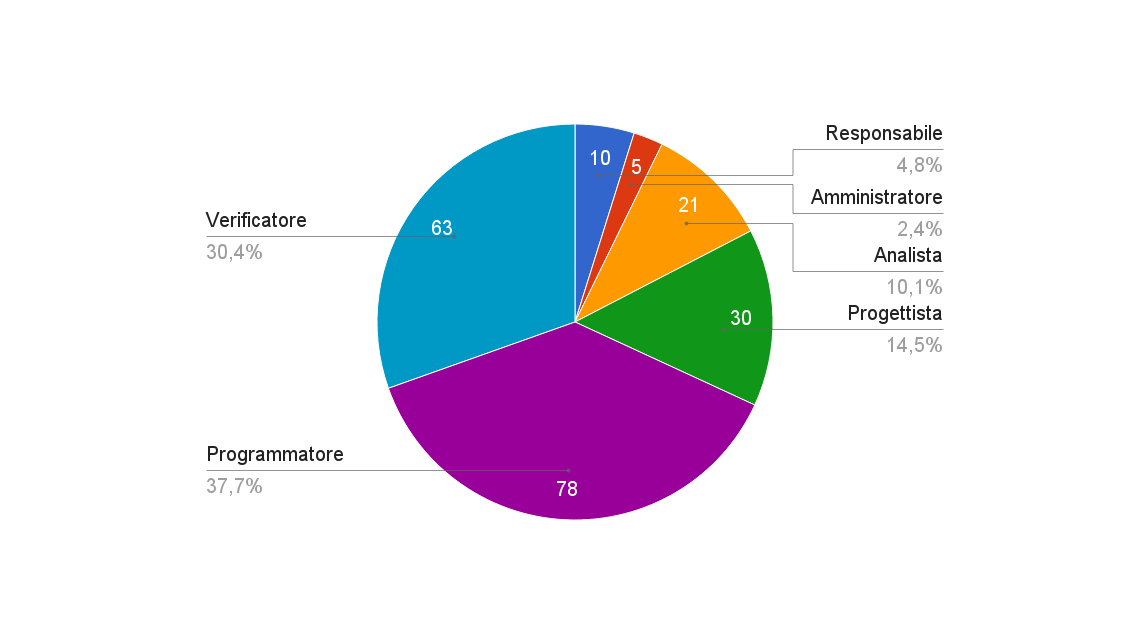
\includegraphics[height=8cm, width=14cm]{img/percOre/PercentualeOreFasePDC.png} 
				\caption{Percentuale di ore per ruolo - Fase PDC}
			\end{figure}
			\newpage
			
				
		
		\subsubsection{Fase RD}	
			\paragraph{Suddivisione del lavoro}
			Nella seguente tabella è descritta la divisione del lavoro nella fase RD:
			\begin{tabella}{!{\VRule}c!{\VRule}c!{\VRule}c!{\VRule}c!{\VRule}c!{\VRule}c!{\VRule}c!{\VRule}c!{\VRule}}
				
				\intestazioneeightcol{Nome}{RE}{AM}{AN}{PG}{PR}{VR}{Ore totali}
				
				Viviana Alessio & - & 3 & 2 & - & - & 5 & 10 \\
				Enrico Bellio & 3 & - & - & 6 & - & 3 & 12 \\
				Matteo Franco & - & - & - & 3 & 10 & - & 13 \\
				Andrea Grendene & - & - & - & - & - & 11 & 11 \\
				Tommaso Panozzo & - & - & - & 5 & 4 & 2 & 11 \\
				Luca Soldera  & - & - & - & - & 12 & - & 12 \\
				
				\hiderowcolors
				\caption{Ore per componente - Fase RD}
				
			\end{tabella}
			\newpage
			
			\ist{img/istogrammiOre/istRD}{Istogramma ruoli - Fase RD}

			
			\paragraph{Prospetto economico}
			Nella seguente tabella sono riportati i costi relativi alla fase RD da rendicontare al Proponente: 
			\begin{tabella}{!{\VRule}c!{\VRule}c!{\VRule}c!{\VRule}}
				\intestazionethreecol{Ruolo}{Ore}{Costo}
				
				Responsabile & 3 & 90\euro \\
				Amministratore & 3 & 60\euro \\
				Analista & 2 & 50 \\
				Progettista & 14 & 308\euro \\
				Programmatore & 26 & 390\euro \\
				Verificatore & 21 & 315\euro \\
				\hline
				\textbf{Totale} & \textbf{69} & \textbf{1213\euro} \\
				\hiderowcolors
				\caption{Ore per ruolo - Fase RD}
			\end{tabella}
			\newpage
			
			\torta{img/percSoldi/percSoldiRD.png}{Percentuale di costo per ruolo sul totale - Fase RD}	
			\torta{img/percOre/PercentualeOreFaseRD.png}{Percentuale di ore per ruolo sul totale - Fase RD}
			
		
		\subsubsection{Fase V}
			\paragraph{Suddivisione del lavoro}
			Nella seguente tabella è descritta la divisione del lavoro nella fase V:
			\begin{tabella}{!{\VRule}c!{\VRule}c!{\VRule}c!{\VRule}c!{\VRule}c!{\VRule}c!{\VRule}c!{\VRule}c!{\VRule}}
				
				\intestazioneeightcol{Nome}{RE}{AM}{AN}{PG}{PR}{VR}{Ore totali}
				
				Viviana Alessio & - & 3 & 2 & - & - & 5 & 10 \\
				Enrico Bellio & - & 5 & - & - & - & 7 & 12 \\
				Matteo Franco & - & - & - & 3 & - & 7 & 11 \\
				Andrea Grendene & 5 & - & - & - & 6 & - & 11 \\
				Tommaso Panozzo & - & - & - & 5 & 5 & 3 & 13 \\
				Luca Soldera  & - & - & - & - & 5 & 6 & 11 \\
				
				\hiderowcolors
				\caption{Ore per componente - Fase V}
				
			\end{tabella}
			
			\ist{img/istogrammiOre/istRD}{Istogramma ruoli - Fase V}		

			
			\paragraph{Prospetto economico}
			Nella seguente tabella sono riportati i costi relativi alla fase V da rendicontare al Proponente: 
			\begin{tabella}{!{\VRule}c!{\VRule}c!{\VRule}c!{\VRule}}
				\intestazionethreecol{Ruolo}{Ore}{Costo}
				
				Responsabile & 5 & 150\euro \\
				Amministratore & 8 & 160\euro \\
				Analista & 2 & 50\euro \\
				Progettista & 8 & 176\euro \\
				Programmatore & 16 & 240\euro \\
				Verificatore & 29 & 435\euro \\
				\hline
				\textbf{Totale} & \textbf{68} & \textbf{1211\euro} \\
				\hiderowcolors
				\caption{Ore per ruolo - Fase V}
			\end{tabella}
			\newpage
			
			\torta{img/percSoldi/percSoldiV.png}{Percentuale di costo per ruolo sul totale - Fase V}	
			\torta{img/percOre/PercentualeOreFaseV.png}{Percentuale di ore per ruolo sul totale - Fase V}
			\newpage
			
	\subsection{Riepilogo}
		\subsubsection{Ore investite}
		Di seguito un resoconto delle ore investite nella fase non rendicontata.
		
		\begin{tabella}{!{\VRule}c!{\VRule}c!{\VRule}c!{\VRule}c!{\VRule}c!{\VRule}c!{\VRule}c!{\VRule}c!{\VRule}}
			
			\intestazioneeightcol{Nome}{RE}{AM}{AN}{PG}{PR}{VR}{Ore totali}
			
			Viviana Alessio & 12 & 2 & - & - & - & 8 & 22 \\
			Enrico Bellio & - & - & 15 & - & - & 7 & 22 \\
			Matteo Franco & - & 14 & - & - & - & 8 & 22 \\
			Andrea Grendene & - & - & 20 & - & - & 3 & 23 \\
			Tommaso Panozzo & - & 6 & 15 & - & - & 3 & 24 \\
			Luca Soldera  & - & 14 & - & - & - & 8 & 22 \\
			
			\hiderowcolors
			\caption{Ore per componente - Fase non rendicontata}
			
		\end{tabella}
		
		\begin{tabella}{!{\VRule}c!{\VRule}c!{\VRule}c!{\VRule}}
			\intestazionethreecol{Ruolo}{Ore}{Costo}
			
			Responsabile & 12 & 360\euro \\
			Amministratore & 36 & 720\euro \\
			Analista & 50 & 1250\euro \\
			Progettista & - & - \\
			Programmatore & - & - \\
			Verificatore & 37 & 555\euro \\
			\hline
			\textbf{Totale} & \textbf{135} & \textbf{2885\euro} \\
			\hiderowcolors
			\caption{Ore per ruolo - Fase A}
		\end{tabella}
		
		\torta{img/percSoldi/percSoldiA.png}{Percentuale di costo per ruolo sul totale - Fase non rendicontata}	
		\torta{img/percOre/PercentualeOreFaseA.png}{Percentuale di ore per ruolo sul totale - Fase non rendicontata}
		
		
		\subsubsection{Ore rendicontate}
		Di seguito un resoconto delle ore lavorative delle fasi rendicontate.
		
		\begin{tabella}{!{\VRule}c!{\VRule}c!{\VRule}c!{\VRule}c!{\VRule}c!{\VRule}c!{\VRule}c!{\VRule}c!{\VRule}}
			
			\intestazioneeightcol{Nome}{RE}{AM}{AN}{PG}{PR}{VR}{Ore totali}
			
			Viviana Alessio & - & 11 & 24 & 14 & 15 & 38 & 102 \\
			Enrico Bellio & 3 & 10 & 10 & 6 & 23 & 50 & 102 \\
			Matteo Franco & 10 & - & 16 & 37 & 10 & 29 & 102 \\
			Andrea Grendene & 5 & 3 & - & 20 & 31 & 43 & 102 \\
			Tommaso Panozzo & 10 & 5 & 5 & 46 & 24 & 12 & 102 \\
			Luca Soldera  & 5 & 5 & 8 & 35 & 20 & 29 & 102 \\
			
			\hiderowcolors
			\caption{Ore per componente - Fasi rendicontate}
			
		\end{tabella}
		
		\begin{tabella}{!{\VRule}c!{\VRule}c!{\VRule}c!{\VRule}}
			\intestazionethreecol{Ruolo}{Ore}{Costo}
			
			Responsabile & 33 & 990\euro \\
			Amministratore & 34 & 680\euro \\
			Analista & 63 & 1575\euro \\
			Progettista & 158 & 3476\euro \\
			Programmatore & 123 & 1845\euro \\
			Verificatore & 201 & 3015\euro \\
			\hline
			\textbf{Totale} & \textbf{612} & \textbf{11581\euro} \\
			\hiderowcolors
			\caption{Ore per ruolo - Fasi rendicontate}
		\end{tabella}
		
		\torta{img/percSoldi/percSoldiRENDICONTATE.png}{Percentuale di costo per ruolo sul totale - Fasi rendicontate}	
		\torta{img/percOre/PercentualeOreFasiRENDICONTATE.png}{Percentuale di ore per ruolo sul totale - Fasi rendicontate}
		
		
		
	
	
